\documentclass[12pt, a4paper, oneside,titlepage]{article}
\usepackage{geometry}
\usepackage{fullpage}
\usepackage{graphicx}
\usepackage{amssymb}
\usepackage{layout}
\usepackage{epstopdf}
\usepackage{gastex}
\usepackage{multicol}
\usepackage{color}
\usepackage{soul}
\usepackage{hyperref}

\hypersetup{linkbordercolor={0 0.5 1}}

\setlength{\textheight}{58em}
\setlength{\footskip}{5em}

\setlength{\parindent}{0mm}

\frenchspacing

\DeclareGraphicsRule{.tif}{png}{.png}{`convert #1 `dirname #1`/`basename #1 .tif`.png}
\renewcommand{\labelenumi}{(\textit{\alph{enumi}})}
\renewcommand{\labelenumii}{(\textit{\roman{enumii}})}

\begin{document}

 \begin{titlepage}
 \begin{center}
 \textsc{\huge{Project Delta}} \\
 {\Large{An Interactive FPGA Circuit Simulator}}
\end{center}
\vspace{10em}
 \begin{center}
{\huge{Specification}}
\end{center}
\vfill
\setlength{\columnsep}{10em}
\begin{multicols}{2}{
\emph{Developers:}\\
Robert Duncan -- \texttt{rad55@cam.ac.uk} \\
Justus Matthiesen -- \texttt{jm614@cam.ac.uk}\\
David Weston -- \texttt{djw83@cam.ac.uk}\\
Christopher Wilson -- \texttt{cw397@cam.ac.uk}\\
Rubin Xu -- \texttt{rx201@cam.ac.uk}\\
\emph{Client:}\\
Steven Gilham\\
\texttt{steven.gilham@citrix.com}
\\
\\
}
\end{multicols}
\begin{center}
\today
\end{center}
 \end{titlepage}

\tableofcontents
\newpage
\setlength{\parskip}{\medskipamount}
\section{Project description}
It would be useful if a first year computer scientist could rapidly prototype a circuit on an Altera DE2 FPGA board without using a hardware description language. The user interface might be presented as a graphical circuit entry system allowing the user to select components from a library (including, 2- and 3-input NOR and NAND gates, RS-latch and D flip-flop) and place them on the screen. Additional components like RAMs and ROMs would be desirable. Switches and LEDs that are present on the DE2 board should be present in the graphical environment to allow circuits to be interfaced to them. Saving and loading of circuits is desirable. Circuits created should be simulated on the DE2 board. The transfer of the circuit to the FPGA simulation might happen in real-time (i.e. any change in the circuit is reflected "instantly" in the simulation). The simulation might be performed in software by a soft processor on the FPGA. For a high performance implementation, the graphical circuit might also be written out as Verilog and then synthesised for direct implementation on the FPGA.
\section{Proposal}
A Java based solution is proposed with a GUI that allows the user, in this case a first year computer scientist, to design a simple circuit using a drag-and-drop interface. The application will allow the user to send their design to the Altera DE2 board for simulation using a Java-based processor.  What follows is a description of the required features and our plan to implement them within the time restriction given.
\section{Major planned features}
 \label{sec:majfeat}
\begin{enumerate}
\item Tri-state wires: with \texttt{0},\texttt{1}, and \texttt{X} states.
\item A component library containing:	 \begin{enumerate}
								\item NOR gate (2/3 input).
								\item NAND gate (2/3 input).
								\item AND gate (2/3 input).
								\item OR gate (2/3 input).
								\item XOR gate (2/3 input).
								\item XNOR gate (2/3 input).
								 \item NOT gate
								 \item Fixed Input (\texttt{0}/\texttt{1})
								\item RS latch.
								\item D flip-flop.
								\item limited size RAM.
								\item limited size ROM.
								\end{enumerate}
\item The ability to ``connect" circuit to built-in LEDs, toggle switches, and push buttons on DE2 boards.
\item The ability to group and ungroup components into a single composite component.
\item Reasonably accurate simulation of circuit on DE2 board, not withstanding variable gate and wire delay (i.e. only have fixed gate delay equal across all components).
\item Single clock with variable frequency.
\item Components can have multiple wires attached to each output connector, however they may only have one wire for each input connector.  
\item An intuitive GUI with:  \begin{enumerate}
						\item Expandable component library.
						\item Switch/button/LED library. 
						\item Drag-and-drop component placing and wiring.
					    \item Flexible wiring that can attach to input/output connectors on components.
					    \item Undo/redo.
					     \item Copy/paste.
					    	\item Zooming.
						\item Document loading/saving.
						\end{enumerate}
\item Capability to export to verilog to be implemented directly onto the FPGA.
\item Fast transfer of designed circuit to DE2 board to be simulated.
\end{enumerate}

\section{Acceptance criteria}
Even though we will endeavour to complete all the major features listed in section \ref{sec:majfeat}, we may find it necessary to make variations during development of the project. The final project must satisfy the following criteria:
\begin{enumerate}
\item Core GUI.
\item Loading/saving of circuits.
\item At least switch/button/LED connection along with NAND and NOR gates (2/3 input), RS latches and D flip-flops.
\item Simulation of circuit on DE2 board.
\item Clock frequency control.
\end{enumerate}

\section{Circuit description}
A limited number of components are going to represented, trying to fairly represent the knowledge and interests of a first year computer scientist. 

We will be considering the output of all gates to initially be \texttt{X}, and all disconnected wires will also have a value of \texttt{X}. This tri-state approach is necessary to model disconnection of wires, and also to represent an unknown signal on a wire. 

Here follows a description of each component represented in the circuit simulator:

\subsection{Simple gates}
\subsubsection{NOT gate}
A NOT gate is essentially an inverter, negating the input as per this table:
\begin{center}
\begin{tabular}{l |c}
$x$ & \texttt{NOT}$(x)$\\
\hline
\texttt{0} & \texttt{1}\\
\hline
\texttt{1} & \texttt{0}\\
\hline
\texttt{X} & \texttt{X}\\
\hline
\end{tabular}
\end{center}
where $x$ is the input to the NOT gate. 

\subsubsection{AND and NAND gates}
A two input AND can be desribed with the following table in our tri-state logic:
\begin{center}
\begin{tabular}{c |l  l l}
\texttt{AND} & \texttt{0} & \texttt{1} & \texttt{X}\\
\hline
\texttt{0} & \texttt{0} & \texttt{0} & \texttt{0}\\
\hline
\texttt{1} & \texttt{0} & \texttt{1} & \texttt{X}\\
\hline
\texttt{X} & \texttt{0} & \texttt{X} & \texttt{X}\\
\hline
\end{tabular}
\end{center}
A three input AND could be modelled as $y = ((x_1\ \texttt{AND}\ x_2)\ \texttt{AND}\ x_3)$ where $x_n$ are inputs to the AND gate, and $y$ is the output. 

A NAND gate has exactly this behaviour except the output, $y$, is inverted, as if it were by a NOT gate. 


\subsubsection{OR and NOR gates}
A two input OR can be desribed with the following table in our tri-state logic:
\begin{center}
\begin{tabular}{c |l  l l}
\texttt{OR} & \texttt{0} & \texttt{1} & \texttt{X}\\
\hline
\texttt{0} & \texttt{0} & \texttt{1} & \texttt{X}\\
\hline
\texttt{1} & \texttt{1} & \texttt{1} & \texttt{1}\\
\hline
\texttt{X} & \texttt{X} & \texttt{1} & \texttt{X}\\
\hline
\end{tabular}
\end{center}
A three input OR could be modelled as $y = ((x_1\ \texttt{OR}\ x_2)\ \texttt{OR}\ x_3)$ where $x_n$ are inputs to the OR gate, and $y$ is the output. 

A NOR gate has exactly this behaviour except the output, $y$, is inverted, as it were by a NOT gate. 

\subsubsection{XOR and XNOR gates}
A two input OR can be desribed with the following table in our tri-state logic:
\begin{center}
\begin{tabular}{c |l  l l}
\texttt{XOR} & \texttt{0} & \texttt{1} & \texttt{X}\\
\hline
\texttt{0} & \texttt{0} & \texttt{1} & \texttt{X}\\
\hline
\texttt{1} & \texttt{1} & \texttt{0} & \texttt{1}\\
\hline
\texttt{X} & \texttt{X} & \texttt{1} & \texttt{X}\\
\hline
\end{tabular}
\end{center}
A three input XOR could be modelled as $y = ((x_1\ \texttt{XOR}\ x_2)\ \texttt{XOR}\ x_3)$ where $x_n$ are inputs to the OR gate, and $y$ is the output. 

An XNOR gate has exactly this behaviour except the output, $y$, is inverted, as if it were by a NOT gate. 

\subsection{Further components}
\subsubsection{Clock}
Each circuit will have a single clock associated with it, that is automatically tied to each clock input on any clocked components. The Clock will have a customisable frequency that is some multiple of the simulation time quantum. 
\subsubsection{D flip-flop}
A D flip flop can be represented using a state transition table, where $Q'$ represents the output $Q$ after a clock tick:

\begin{center}
\begin{tabular}{c |c | c}
$D$ & $Q$ & $Q'$\\
\hline
\texttt{0} & \texttt{Q} & \texttt{0}\\
\texttt{1} & \texttt{Q} & \texttt{1}\\
\texttt{X} & \texttt{Q} & \texttt{X}\\
\end{tabular}
\end{center}
We will be using single output D flip-flops, i.e. they will not contain an extra negated output. This doesn't affect the potential set of circuits though, since a user can attach multiples wires to a single output.
\subsubsection{RS Latch}
This a grouped component described by the following table: \\
\hl{I'm not sure this table is correct}
\begin{center}
\begin{tabular}{c |c | c | c}
$R$ & $S$ & $Q$ & $\overline{Q}$\\
\hline
\texttt{0} & \texttt{0} & \texttt{Q} & $\overline{\texttt{Q}}$\\
\texttt{0} & \texttt{1} & \texttt{1} & \texttt{0}\\
\texttt{1} & \texttt{0} & \texttt{0} & \texttt{1}\\
\texttt{1} & \texttt{1} & \texttt{U} & \texttt{U}\\
\texttt{0} & \texttt{X} & \texttt{X} & \texttt{X}\\
\texttt{X} & \texttt{0} & \texttt{X} & \texttt{X}\\
\texttt{1} & \texttt{X} & \texttt{X} & \texttt{X}\\
\texttt{X} & \texttt{1} & \texttt{X} & \texttt{X}\\
\texttt{X} & \texttt{X} & \texttt{X} & \texttt{X}\\
\end{tabular}
\end{center}
Where \texttt{U} stands for unstable. This conbination of inputs is to be avoided if at all possible.

\subsubsection{ROM and RAM}
Whilst we don't provide the ability to use buses natively, they can be constructed from groups of wires. With both ROM and RAM the user will be able to preset the contents in the GUI before loading it to the DE2 board. 

However, ROMs will not have the ability to set the contents of the cell when addressing it, only to read out the contents. 

\begin{enumerate}
\item 16 cells, addressable with 4 address inputs.
\item Each cell stores a single boolean value. 
\item RAM has a write enable input along with a data input.
\item A single output wire with the data contained at the addressed wire. 
\item an implicit clock connection, so that reads and write only occur on clock pulses.
\end{enumerate}

\subsection{Inputs and outputs}
\subsubsection{LEDs}
These can be used within the circuit and they correspond to a labelled LED on the physical hardware.
\subsubsection{Switches and buttons}
These can be used within the circuit and they correspond to the labelled switch or button on the physical hardware. 

\section{Data structure}
\label{sec:datastruct}
This section contributed by Justus Matthiesen.

\section{Simulation algorithm}
This section contributed by Justus Matthiesen. 

\section{Using the Altera DE2 board}
\subsection{Java processor}
The simulation program will be written in Java and executed on an open-source Java bytecode processor, \emph{JOP}\footnote{JOP: A Tiny Java Processor Core for FPGA \url{http://www.jopdesign.com/}}, running on the Altera DE2 board. The \emph{JOP} is a RISC processor with its own stack-based microcode instruction set. Java bytecode is translated into the corresponding microcode(s) during the decode stage of the processor cycle. A real-time garbage collector is implemented in Java, compiled as part of the target Java application and is invoked by the processor when necessary. All IO devices are integrated as memory-mapped devices into the uniform address space, distinguishing themselves from RAM spaces using the highest two bits of the address line. \emph{JOP} provides a pre-existing toolchain to compile and run Java programs onto the DE2 board, thus enabling more time to spent on the GUI and the simulation program that will run on the board. 

Access to the DE2 board's LEDs and switches can be made through memory-mapped IO. Simple Java wrapper classes can be used to present an abstracted interface to the simulation program. 

Access to the SDRAM provided by the board (8MB) can be provided with a adapted open-source SDRAM controller\footnote{Altera DE2 SDRAM Controller \url{http://whoyouvotefor.info/altera_sdram.html}} for the Altera DE2 board. This access will be multiplexed with the access to the faster SRAM (512KB) to provided a unified address space that can be access from a Java interface. 

\subsection{Communication}
A serial connection is already provided for within the \emph{JOP} toolchain, a datagram layer can be adapted from the JOP libraries to provide a packetised interface to and from the board that is suited to the needs of the application. On top of this datagram layer, a serialized object channel will be used to communicate the circuit design from the GUI to the simulation program running on the board. 

There is the possibility of emulating the serial connection using the USB blaster connection to avoid having two cables between the board and the computer used for the design work. However, at the moment only one-way connection (to the computer from the board) on the USB cable has been achieved. 

This section contributed by Rubin Xu.



\section{Exporting to Verilog}
Exporting the circuit description to Verilog means that our GUI application to design circuits can be used independently of the DE2 board. This enables a huge variety of hardware devices to be used with our application other than the DE2 board. It also allows for faster circuit simulation than using the \emph{JOP} on the board, allowing for more realistic simulation. 

Verilog modules will be used to describe the D flip-flop, RS latch, RAM, and the ROM components. Using structural Verilog to describe the structure of the circuit, the application will be able to quickly produce Verilog descriptions from the internal data structure described in section \ref{sec:datastruct}.

We will not implement a software component to send the Verilog to the board within the application, instead producing a Verilog \texttt{.v} source file to retain greater flexibility in the destination of the Verilog description. 

\section{GUI}
\begin{figure}[h]
\centering
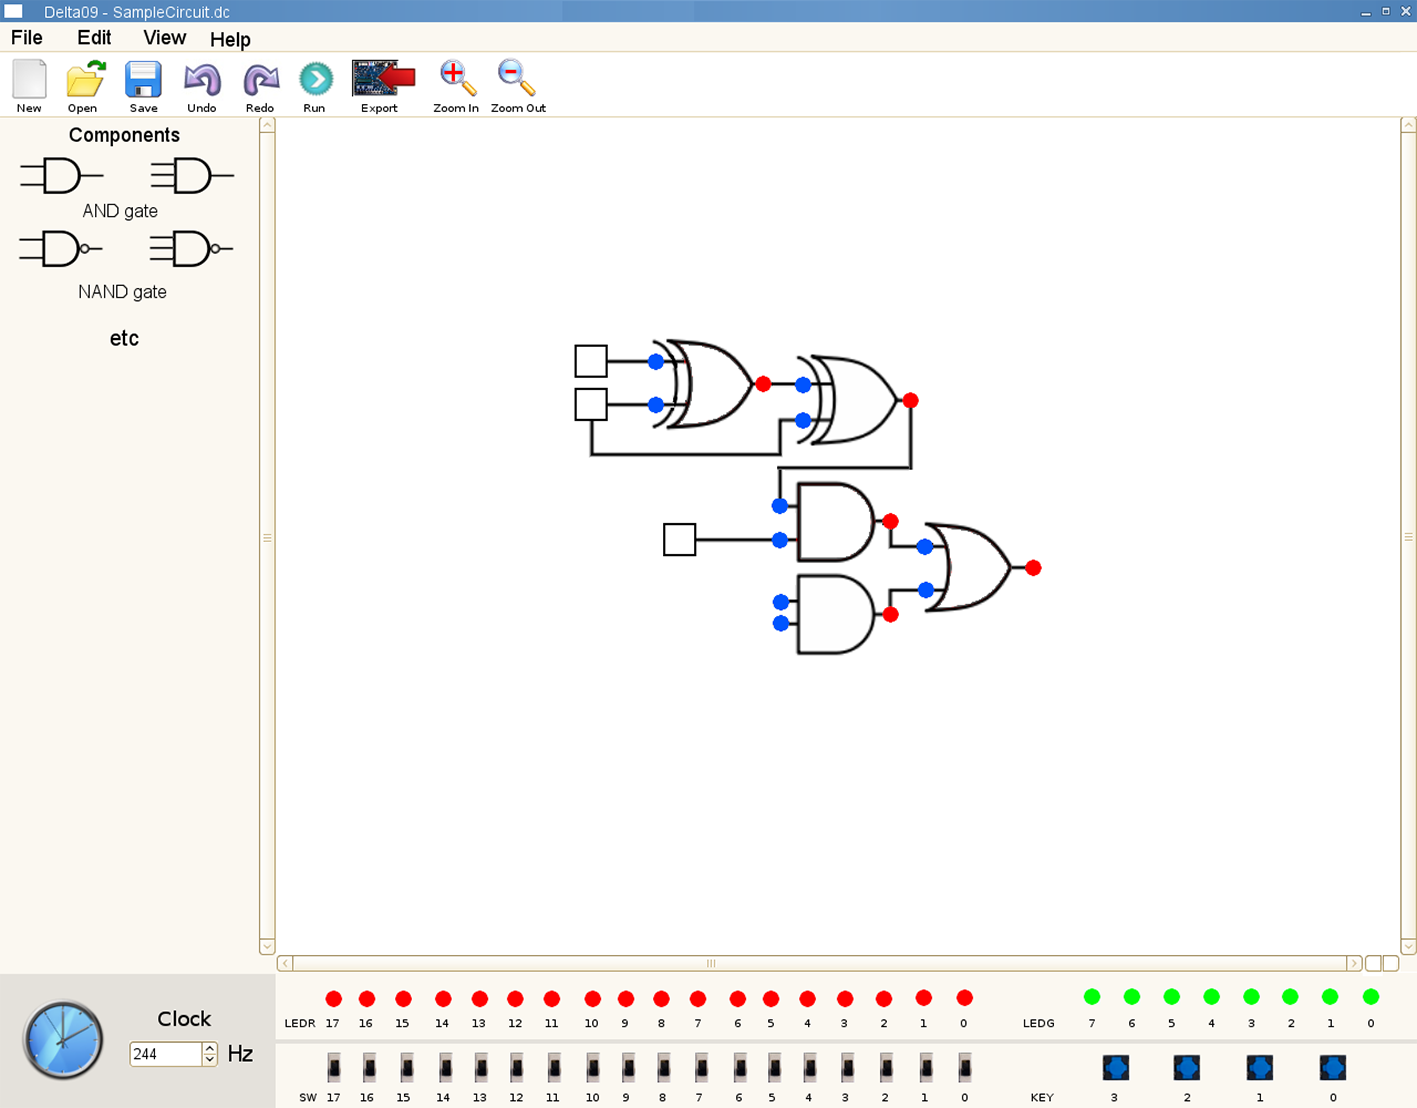
\includegraphics[width=12cm]{GUI_mockup.png}
\caption{Mockup of graphical interface}\label{fig:erptsqfit}
\end{figure}
The user interface will consist of the following elements:
\begin{enumerate}
\item A scrollable main panel where the circuit to be simulated is designed.
\item A scrollable panel to the left of this, which contains a list of circuit components (gates, ROM/RAM, RS-latch, D-flip-flop, fixed inputs) with graphics and text descriptions.
\item A panel underneath the main one containing diagramatic representations of all the DE2 board's toggle switches, push-buttons and red and green LEDs.
\item A panel in the bottom-left corner of the window containing a clock icon and an adjustable frequency spinner.
\item A toolbar at the top of the window containing: \begin{enumerate}
												\item New circuit.
												\item Load circuit.
												\item Save circuit.
												\item Undo.
												\item Redo.
												\item Transfer to board.
												\item Export to Verilog.
												\item Zoom in.
												\item Zoom out.
												\end{enumerate}
												
\item A menu bar containing the following menus: \begin{enumerate}
												\item File
												\begin{enumerate}
												\item New.
												\item Open.
												\item Save.
												\item Exit.
												\end{enumerate}																											\item Edit
																								\begin{enumerate}
												\item Undo.
												\item Redo.
												\item Cut.
												\item Copy.
												\item Paste.
												\item Delete.
												\end{enumerate}		
												
												 \item View
												 												\begin{enumerate}
												\item Zoom in.
												\item Zoom out.
												\end{enumerate}	
												
												 \item Help
												 												\begin{enumerate}
												\item Contents.
												\item About.
												\end{enumerate}	
												\end{enumerate}

\end{enumerate}
The user should be able to drag components from the left or bottom panels and drop them in the main panel to form part of the circuit. The interface will allow unlimited uses of each type of component with the exception of the LEDs, which are single-use only. Each component in the main panel will have one or more ports for input (represented as blue circles) and/or output (represented as red circles). Wires will be constructed by clicking on one of these ports, followed by clicking on a port of the opposite type. The interface will disallow multiple wires being connected to the same input port, and wires being connected from one input port to another (and similarly with output ports). The user will be able to select intermediate points for the wires by clicking as many times as desired between the source and destination ports.


The user should be able to select components and wires in the main panel by clicking on them, which will highlight them. Multiple components and wires will be selected by dragging out a box. Selections can be moved by dragging. They can also be cut, copied, pasted and deleted using the edit menu, buttons on the toolbar or keyboard shortcuts.

The user will be able to change the size and position of the display of the circuit by zooming (using the toolbar/menu bar controls) and scrolling.

The current circuit will be simulated on the board when the user clicks the "transfer to board" button. This will then be greyed out until a change is made to the circuit.

This section contributed by Christopher Wilson and David Weston.

\section{Distribution of responsibility}
The r\^oles defined here are \hl{temporary} assignments. \\ \\ 
\begin{tabular}{l l}
Robert Duncan & Data Structure \& Integration\\ 
Justus Matthiesen & Simulator \\
David Weston & GUI \\
Christopher Wilson & GUI \\
Rubin Xu & Hardware \\
\end{tabular}

\end{document}  